\documentclass[tikz,border=8pt]{standalone}
\usepackage[T1]{fontenc}
\usepackage{newtxtext,newtxmath}
\usetikzlibrary{arrows.meta,positioning}
\definecolor{inkblue}{RGB}{40,83,123}
\definecolor{inkgreen}{RGB}{48,112,94}
\begin{document}
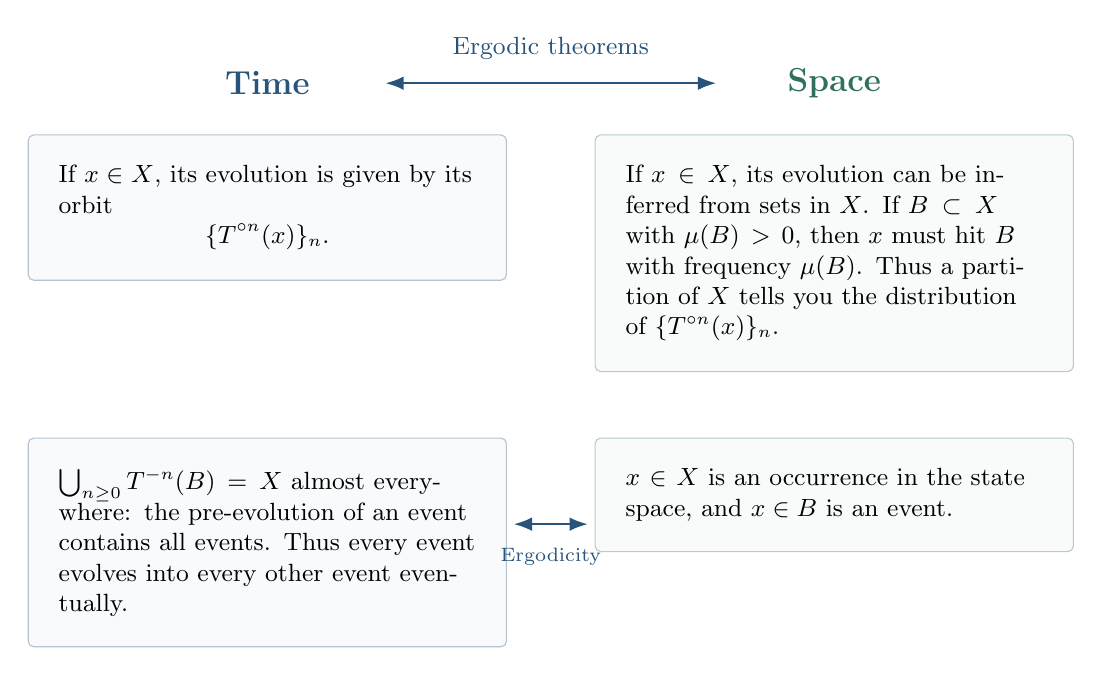
\begin{tikzpicture}[>=Latex,font=\small,
  box/.style={draw=inkblue!35,rounded corners=2pt,fill=inkblue!3,
  text width=5.3cm,align=left,inner sep=11pt}]
  \node[font=\large\bfseries,text=inkblue] at (0,0) {Time};
  \node[font=\large\bfseries,text=inkgreen] at (7.2,0) {Space};
  \draw[<->,thick,inkblue] (1.5,0)--(5.7,0)
    node[midway,above=5pt,font=\small] {Ergodic theorems};
  \node[box,anchor=north] (time1) at (0,-.65)
    {If $x\in X$, its evolution is given by its orbit
    \[\{T^{\circ n}(x)\}_n.\]};
  \node[box,anchor=north,draw=inkgreen!35,fill=inkgreen!3] (space1) at (7.2,-.65)
    {If $x\in X$, its evolution can be inferred from sets in $X$.
    If $B\subset X$ with $\mu(B)>0$, then $x$ must hit $B$ with frequency
    $\mu(B)$. Thus a partition of $X$ tells you the distribution of
    $\{T^{\circ n}(x)\}_n$.};
  \node[box,anchor=north] (time2) at (0,-4.5)
    {$\bigcup_{n\geq0}T^{-n}(B)=X$ almost everywhere: the pre-evolution of an event contains
    all events. Thus every event evolves into every other event eventually.};
  \node[box,anchor=north,draw=inkgreen!35,fill=inkgreen!3] (space2) at (7.2,-4.5)
    {$x\in X$ is an occurrence in the state space, and $x\in B$ is an event.};
  \draw[<->,thick,inkblue] (3.13,-5.6)--(4.07,-5.6)
    node[midway,below=5pt,font=\scriptsize] {Ergodicity};
\end{tikzpicture}
\end{document}
